\chapter{Teoría de promediación}

Como vimos, determinar la existencia y propiedades cualitativas y cuantitativas
de los ciclos límite en sistemas no lineales no es tarea fácil. En muchos
casos, los métodos analíticos fallan o se vuelven sumamente complejos, y los
métodos numéricos pueden ser ineficientes o inexactos \cite{guckenheimer1983nonlinear}. \\

El Método de Promediación es una herramienta poderosa y efectiva,
parte de la teoría de perturbaciones y nos ayuda a simplificar el análisis
de sistemas no lineales transformando las ecuaciones originales en un sistema
más manejable. La premisa fundamental es que, bajo ciertas condiciones, el
comportamiento promedio del sistema a lo largo del tiempo puede revelar
la existencia y la estructura de los ciclos límite \cite{hinch1991perturbation}.\\

La aplicación del Método de Promediación para verificar la existencia de
ciclos límite en sistemas no lineales no solo proporciona una técnica
analítica robusta, sino que también ofrece una perspectiva más profunda
del comportamiento oscilatorio inherente en dichos sistemas. Este enfoque
no solo permite simplificar las ecuaciones diferenciales originales, sino
también captar la esencia del comportamiento dinámico del sistema,
facilitando así la identificación y caracterización de ciclos límite \cite{bender2013advanced}.\\

Definiendo el promedio local de una función y algunas de sus propiedades.

\section{Método de promediación}

\begin{definition}
	Sea $f:\mathbb{R}\times\mathbb{R}^p\to\mathbb{R}^n$ continua y $T>0$.
	Definimos:
	\[ 
		f_T(t,x)=\frac{1}{T}\int_{0}^{T}f(t+\tau,x)d\tau
	\]
	como el promedio local de $f$ \cite{hinch1991perturbation}.
\end{definition}

La función $f_T(t,x)$ calcula el valor promedio de la función $f(t,x)$ 
respecto a la variable $t$ en el intervalo $[t,t+T]$, visto de otro 
modo, calcula el comportamiento promedio futuro del tiempo $t$ a tiempo $t+T$.\\

\begin{proposition}
	Sea $f:\mathbb{R}\times\mathbb{R}^p\to\mathbb{R}^n$ continua y de periodo $T$ en $t$, entonces
	\[ 
		f_{T(t,x)}=f_0(x)
	\]
\end{proposition}

Si la función a promediar es de Lipschitz, entonces la diferencia entre ambas
funciones está acotada; esto quiere decir que el mapeo del promedio local de 
la función no se aleja demasiado de la función original, solo lo simplifica 
y guarda el comportamiento promedio de la función \cite{bender2013advanced}.
\begin{proposition}
	Si $\phi:\mathbb{R} \to \mathbb{R}$ es de Lipschitz en $\mathbb{R}$ con constante de Lipschitz $\lambda$, entonces
	\[ 
		\|\phi(x)-\phi_{T(x)}|\leq\frac{\lambda T}{2}
	\]
	i.e. $\phi(t)$ es $o(T)$ con respecto a $\phi_{T(x)}$.
\end{proposition}

\begin{example}
	Consideremos la función $\phi(t)=\sqrt{t^2+1}$, esta función es de Lipschitz
	con constante $\lambda=1$, calculamos su promedio local con $T=0.5$
	\[ 
	\phi_T(t)=\frac{1}{2T}(((T + t)\sqrt{1 + (T + t)^2} + \sinh^{-1}(T + t)) - (t\sqrt{1 + t^2} + \sinh^{-1}(t)))
	\]
	graficamos ambas funciones.

	\begin{figure}[h]
		\centering
		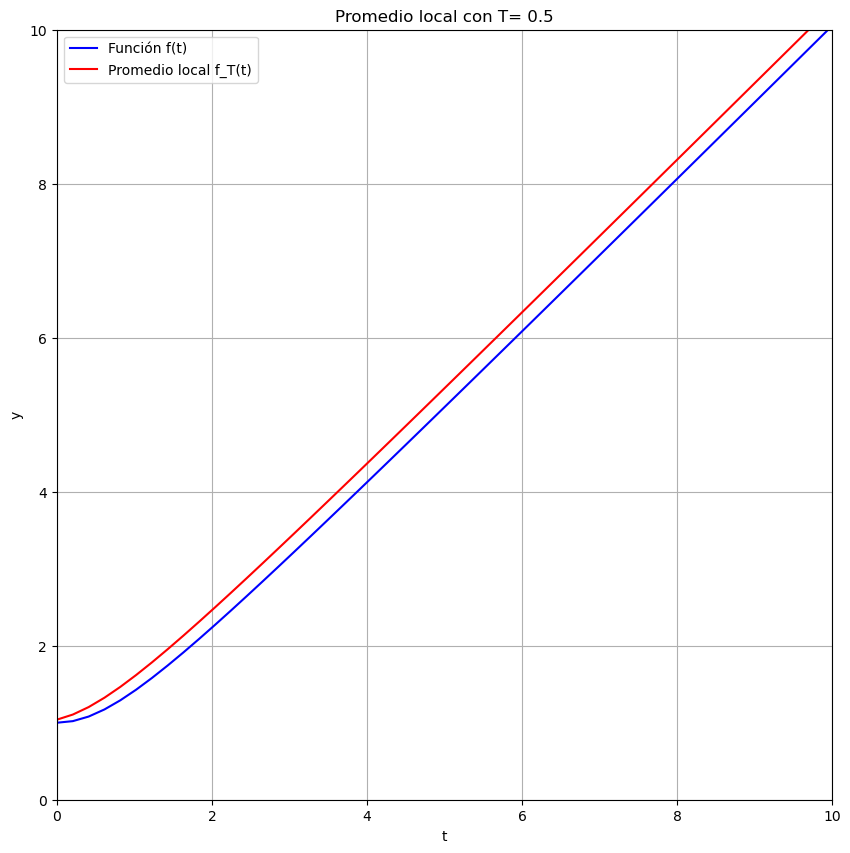
\includegraphics[width=10cm]{fl.png}
		\caption{Función vs función promediada.}
	\end{figure}

	La diferencia está acotada por $M=\frac{\lambda T}{2}=0.25$. En este caso, en la
	gráfica se puede observar que la diferencia converge a la cota $M$.

	\begin{figure}[h]
		\centering
		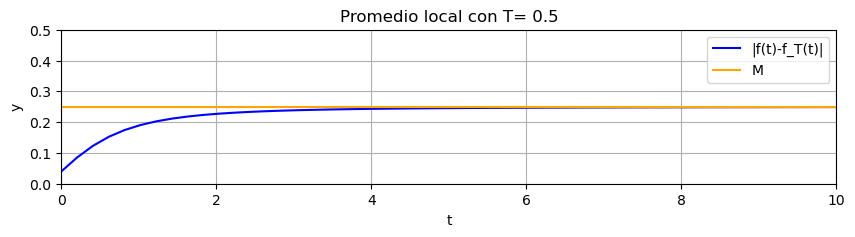
\includegraphics[width=13cm]{d.png}
		\caption{Diferencia de la Función con la función promediada.}
	\end{figure}

\end{example}

\newpage

Este comportamiento asintótico no necesariamente ocurre siempre; un ejemplo es la función $\sin(x)$. 

\begin{lemma}
	Consideremos la EDO
	\[ 
		x'=\epsilon f(t,x)
	\]
	con $x(0)=x_0$, donde $f$ es de Lipschitz en $x\in D\subseteq\mathbb{R}^n$
	y $f$ continua en $t\in[0,t]$.\\
	Sea $M=\sup_{x\in D} \sup_{0\leq\epsilon t\leq L} |f(t,x)|<+\infty$
	\\Si $\phi(t)=\int_{0}^{t}f(\tau,x(\tau))d\tau$ con $x$ solución de la EDO..
	\\Entonces:
	\[ 
		|\phi_T(t)-\int_{0}^{t}f_T(\tau,x(\tau))d\tau|\leq\frac{1}{2}(1+\lambda L)MT
	\]
	para $o(\frac{1}{\epsilon})=t$, donde $\lambda\equiv cte$ de Lipschitz.
	\\i.e. $\phi_T(t)=\int_{0}^{t}f_T(\tau,x(\tau))d\tau+o(T)$
\end{lemma}

\begin{lemma}
	Consideremos el problema de valor inicial
	\[ 
		x'=\epsilon f(t,x)
	\]
	$x(0)=x_0$, con $f$ Lipschitz en $x\in D\subseteq\mathbb{R}^n$ y continua
	en $t\in[0,t]$. \\
	Si $y$ es solución de $y'=\epsilon f_T(t,y)$, $y(0)=x_0$, entonces
	\[ 
		x(t)-y(t)=o(\epsilon T)
	\]
	p.t. $t=o(\frac{1}{\epsilon})$
\end{lemma}

\begin{theorem}
	Consideremos $x'=\epsilon f(t,x)$, $x(t_0)=x_0$ y $y'=f^0(y)$, $y(t_0)=x_0$,
	donde $x_0,x,y\in D\subseteq\mathbb{R}^n$ y $\epsilon\in[0,\epsilon_0]$.\\

	Satisfaciendo:
	\begin{enumerate}
		\item $\bar{f}(t,x)$ es $T$ periódica con promedio $f^0(x)$.
		\item $f$ es continua en $t$ y Lipschitz en $x\in D$.
		\item $y(t)$ permanece en el interior de $D$ para todo $t=O(\frac{1}{\epsilon})$.
	\end{enumerate}
	Entonces
	\[ 
	x(t)-y(t)=O(\delta(\epsilon))
	\]
	para todo $t=o(\frac{1}{\epsilon})$ con $\delta=\delta(\epsilon)$ función de orden.
\end{theorem}

\section{Oscilador de Van der Pol}
De nuevo vamos a trabajar en el Oscilador de Van der Pol, pero ahora vamos a implementar la teoría de promediación para demostrar la existencia de ciclos límite \cite{strogatz2018nonlinear}.\\

Sea el sistema de ecuaciones

\begin{equation}\label{eq: VPsis}
	\begin{matrix}
		y'=-x-\epsilon y(x^2-1) \\ 
		x'=y
	\end{matrix}
\end{equation}

Haremos el cambio de coordenadas a polares.
Sustituimos en $\eqref{eq: dxpolar}$ y $\eqref{eq: dypolar}$ en $\eqref{eq: VPsis}$
$$r\cos(\theta)\theta'+r'\sin(\theta)=-r\cos(\theta)-\epsilon r\sin(\theta)(r^2\cos^2(\theta)-1)$$
$$-r\sin(\theta)\theta'+r'\cos(\theta)=r\sin(\theta)$$
entonces
\begin{equation}\label{eq: VPdr}
	r'=-\epsilon r\sin^2(\theta)(r^2\cos^2(\theta)-1)
\end{equation}
\begin{equation}\label{eq: VPdtheta}
	\theta'=-1-\epsilon r\sin(\theta)\cos(\theta)(r^2\cos(\theta^2)-1)
\end{equation}
Definimos para $\eqref{eq: VPdr}$ el promedio
\begin{equation}\label{eq: drbar}
	\bar{r}'=\bar{f}(\bar{r},\epsilon)
\end{equation}

donde
$$\bar{f}(\bar{r},\epsilon)=\frac{1}{2\pi}\int\limits_0^{2\pi}r'd\theta$$
Calculamos esta integral
$$\bar{f}(\bar{r},\epsilon)=\frac{1}{2\pi}\int\limits_0^{2\pi}-\epsilon r\sin^2(\theta)(r^2\cos^2(\theta)-1)d\theta$$
$$=\frac{1}{2\pi}[-\epsilon r^3\int\limits_0^{2\pi}\sin^2(\theta)\cos^2(\theta)d\theta+\epsilon r\int\limits_0^{2\pi}\sin^2(\theta)d\theta]$$
$$=\frac{1}{2\pi}[-\epsilon r^3[\frac{1}{32}(4\theta-\sin(4\theta))]_0^{2\pi}+\epsilon r[\frac{1}{2}(\theta-\sin(\theta)\cos(\theta))]_0^{2\pi}]$$
$$=\frac{1}{2\pi}[\frac{-\epsilon r^3}{32}(8\pi)+\frac{\epsilon r}{2}(2\pi)]=\frac{1}{2\pi}[\frac{-\epsilon r^3}{4}\pi+\epsilon r\pi].$$
Entonces
$$\bar{f}(\bar{r},\epsilon)=\frac{\epsilon r}{2}-\frac{\epsilon r^3}{8}$$
Promediamos $\theta$
$$\bar{\theta}=2\pi t$$
Vamos a analizar $\eqref{eq: drbar}$
\begin{equation}\label{eq: drvander}
	\bar{r}'=\frac{\epsilon}{8}r(4-r^2)
\end{equation}

\begin{figure}[h]
	\centering
	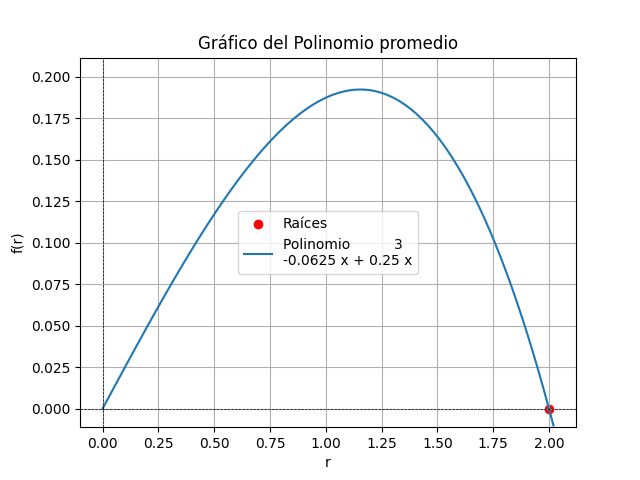
\includegraphics[width=14cm]{graficavanderpol.png}
	\caption{Plano fase de $\eqref{eq:drvander}$.}
\end{figure}
Las soluciones de equilibrio son $r=0$ y $r=2$.
\begin{enumerate}
	\item Si $0<r<2$, entonces $r'>0$, por lo que $0$ es un punto fuente o repulsivo.
	\item Si $r>2$, entonces $r'<0$, entonces $r=2$ es sumidero o atractor.
\end{enumerate}

\begin{figure}[h]
	\centering
	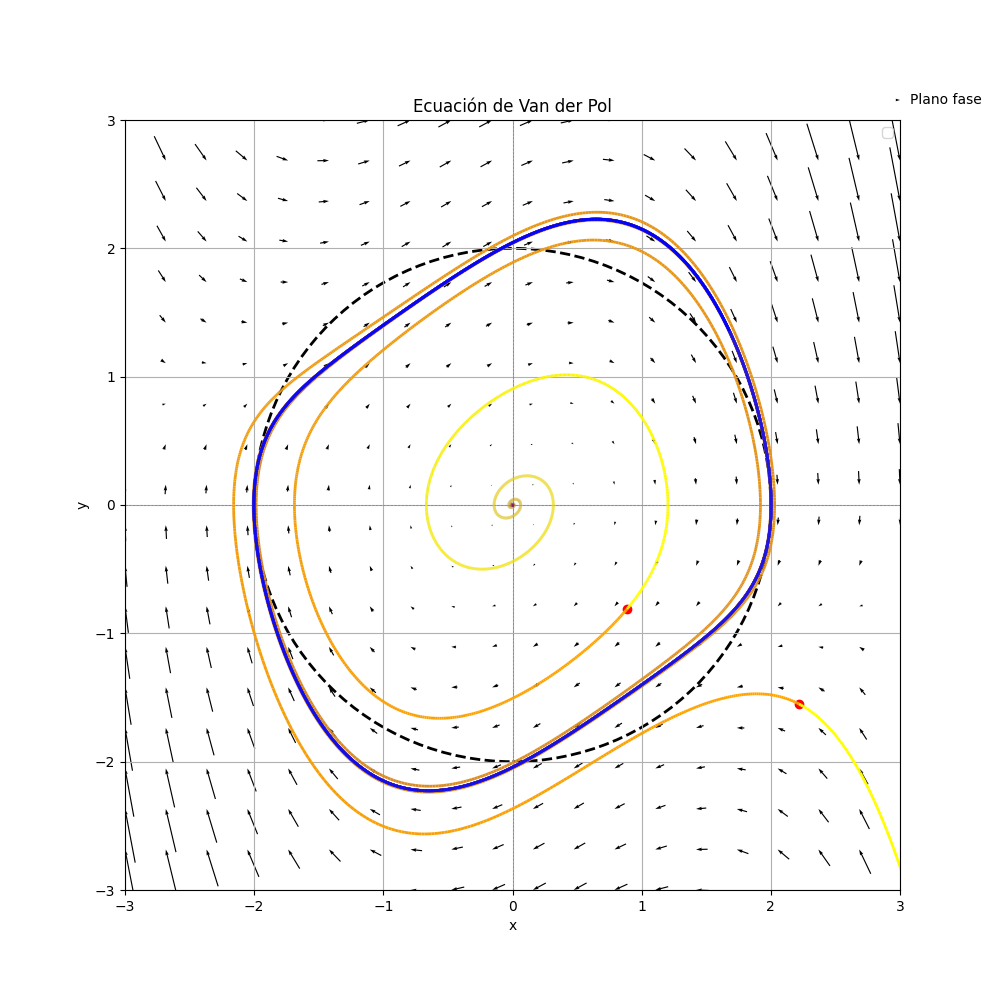
\includegraphics[width=11cm]{vanderpol.png}
	\caption{Plano fase. Dibujado en \href{https://aeb019.hosted.uark.edu/pplane.html}{https://aeb019.hosted.uark.edu/pplane.html}}
\end{figure}

Esto quiere decir que entre dos circunferencias de radios $0<r_{min}<2$ y $2<r_{max}$
existe al menos una curva cerrada a la cual las curvas convergen.

\newpage

\section{Ecuación de Rayleigh}

Vamos a implementar en la ecuación de Rayleigh la teoría de promediación para demostrar la existencia de ciclos límite \cite{strogatz2018nonlinear}.

\begin{equation}\label{eq: Rayleigh}
	\begin{matrix}
		y'=-\epsilon(y^2-1)y-x \\ 
		x'=y
	\end{matrix}
\end{equation}

Haremos el cambio de coordenadas a polares.
$$r\cos(\theta)\theta'+r'\sin(\theta)=-\epsilon (r^2\sin^2(\theta)-1)r\sin(\theta)-\omega^2r\cos(\theta) $$
$$-r\sin(\theta)\theta'+r'\cos(\theta)=r\sin(\theta)$$
Obtenemos la ecuación.
\begin{equation}\label{eq: Rayleighpolar}
	r'=\epsilon(1-r^2\sin^2(\theta))r\sin^2(\theta)+r\sin(\theta)\cos(\theta)(1-\omega^2)
\end{equation}
Definimos para $\eqref{eq: Rayleighpolar}$ el promedio
$$\bar{r}=\bar{f}(\bar{r},\epsilon)=\frac{1}{2\pi}\int\limits_0^{2\pi}r'd\theta$$
Calculamos esta integral
$$\bar{f}(\bar{r},\epsilon)=\frac{1}{2\pi}\int\limits_0^{2\pi}[\epsilon(1-r^2\sin^2(\theta))r\sin^2(\theta)+r\sin(\theta)\cos(\theta)(1-\omega^2)]d\theta$$
$$=\frac{1}{2\pi}\epsilon r\int\limits_0^{2\pi}\sin^2(\theta)d\theta-\frac{1}{2\pi}\epsilon r^3\int\limits_0^{2\pi}\sin^4(\theta)d\theta+\frac{1}{2\pi}r(1-\omega^2)\int\limits_0^{2\pi}\cos(\theta)\sin(\theta)d\theta$$
$$=\frac{1}{2\pi}\epsilon r[\frac{1}{2}(\theta-\sin(\theta)\cos(\theta))]\Big|_2^{2\pi}-\frac{1}{2\pi}\epsilon r^3[\frac{1}{32}(-8\sin(2\theta)+\sin(4\theta)+12\theta)]\Big|_0^{2\pi}+$$
$$\frac{1}{2\pi}r(1-\omega^2)[\cos^2(\theta)]\Big|_0^{2\pi}]=\frac{1}{2\pi}\epsilon r\pi-\frac{1}{2\pi}\epsilon r^3\frac{3}{4}\pi$$
$$=\frac{\epsilon r}{8}(4-3r^2)$$
Entonces tenemos el sistema
$$\bar{r}'=\frac{\epsilon r}{8}(4-3r^2)$$
$$\bar{\theta}'=2\pi t$$

Las soluciones de equilibrio son $r=0$ y $r=\frac{2}{3}\sqrt{3}$
\begin{figure}[h]
	\centering
	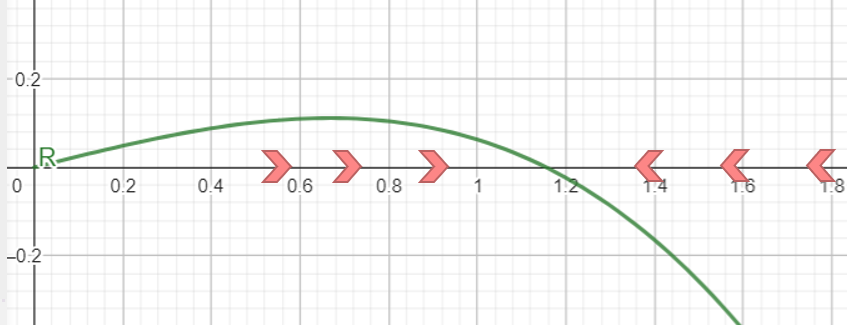
\includegraphics[width=9cm]{graficarayleigh.png}
	\caption{Plano fase.Dibujado en https://aeb019.hosted.uark.edu/pplane.html}
\end{figure}
\begin{figure}[h]
	\centering
	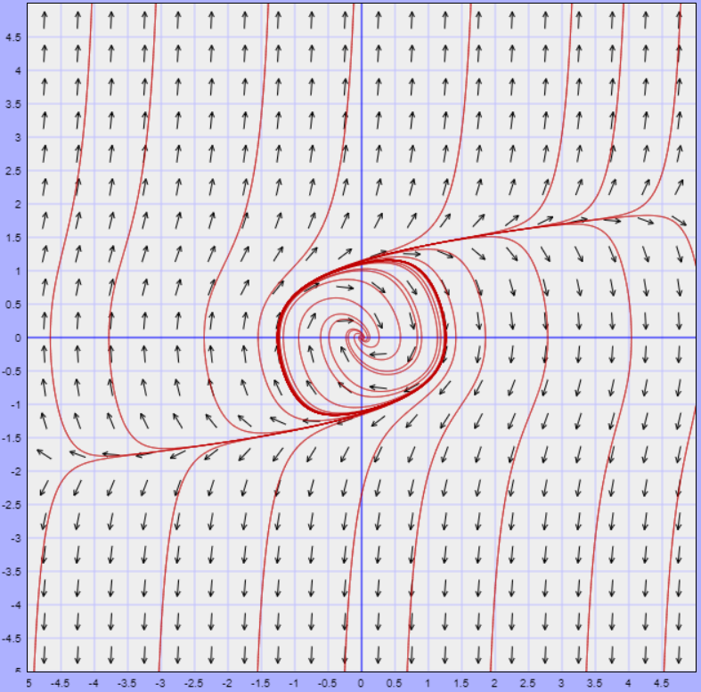
\includegraphics[width=11cm]{planorayleigh.png}
	\caption{Plano fase.Dibujado en https://aeb019.hosted.uark.edu/pplane.html}
\end{figure}

\newpage

\section{Van der Pol y Rayleigh}
Ahora vamos a analizar la EDO
\begin{equation}\label{eq: vdpr}
	x''+\epsilon(x'^2-1)x'+\eta(x^2-1)x'+x=0
\end{equation}
Extendemos esta ecuación a un sistema de ecuaciones haciendo el
cambio de variable usual $y=x'$. Obtenemos lo siguiente:
\begin{equation}\label{eq: vpdrsis}
	\begin{matrix}
		y'=-\epsilon(y^2-1)x'-\eta(x^2-1)y-x \\ 
		x'=y
	\end{matrix}
\end{equation}

Hacemos un cambio de coordenadas a polares. Sustituimos $\eqref{eq: dxpolar}$ y
$\eqref{eq: dypolar}$ en nuestro sistema, obtenemos:
$$r'\sin(\theta)+\theta'r\cos(\theta)=-\epsilon(r^2\sin^2(\theta)-1)r\sin(\theta)-\eta(r^2\cos^2(\theta)-1)r\sin(\theta)-r\cos(\theta)$$
$$r'\cos(\theta)-\theta'r\sin(\theta)=r\sin(\theta)$$
Calculamos $r'$ y $\theta'$
\begin{equation}\label{eq: drvdpr}
	r'=-[\epsilon(r^2\sin^2(\theta)-1)+\eta(r^2\cos^2(\theta)-1)]r\sin^2(\theta)
\end{equation}
$$\theta'=-[\epsilon(r^2\sin^2(\theta)-1)+\eta(r^2\cos^2(\theta)-1)]\cos(\theta)\sin(\theta)-r$$
Vamos a promediar $r'$, calculamos $\bar{r}'$:
$$\bar{r}'=\frac{1}{2\pi}\int_0^{2\pi}-[\epsilon(r^2\sin^2(\theta)-1)+\eta(r^2\cos^2(\theta)-1)]r\sin^2(\theta)d\theta$$
$$=-\frac{r^3}{8}(3\epsilon+\eta)+\frac{r}{2}(\epsilon+\eta)$$
Calculamos las raíces no negativas de $\bar{r}'=-r^3(\frac{3\epsilon+\eta}{8})+r(\frac{\epsilon+\eta}{2})$, estas son
$r_1=0$ y $r_2=2\sqrt{\frac{\epsilon+\eta}{3\epsilon+\eta}}$.\\
\\Para los valores de $\epsilon=0.5$ y $\eta=0.4$ el valor del atractor es $r_2=1.3764\dots$, podemos ver en la imagen que en efecto
existe un ciclo límite aproximado a la circunferencia de radio $r_2$.

\begin{figure}[h]
	\centering
	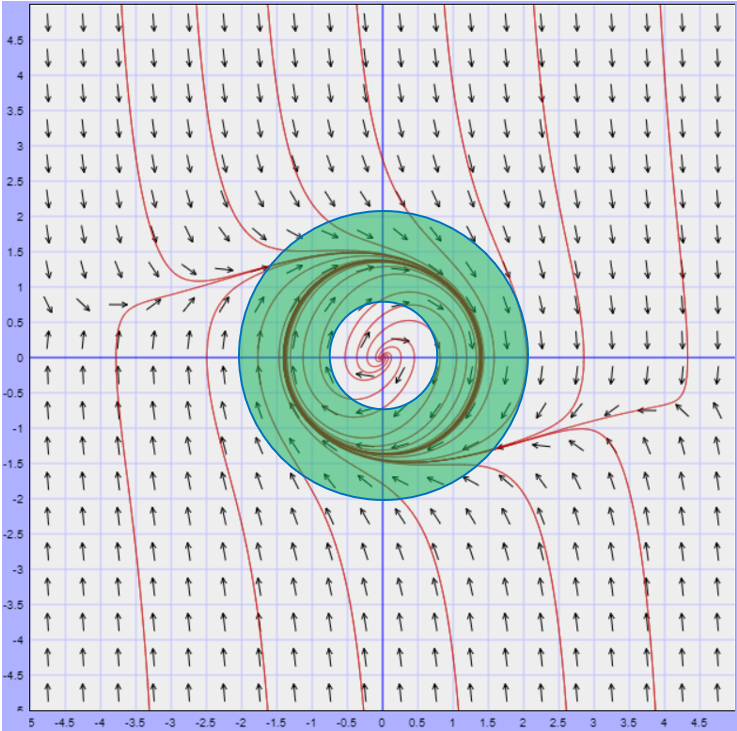
\includegraphics[width=9cm]{VDP-R.png}
	\caption{Plano fase.Dibujado en \href{https://aeb019.hosted.uark.edu/pplane.html}{https://aeb019.hosted.uark.edu/pplane.html}}
\end{figure}
\newpage
